% !TEX TS-program = XeLaTeX
% !TEX spellcheck = en-US
\documentclass[aspectratio=169]{beamer}
\usepackage{tikz}
\usetikzlibrary{positioning}

\usetheme{example}

\title{Lecture 8:\\ Backpropagation and Gradient Descent}
\institute{GRA4160: Predictive modelling with machine learning}
\date{February 27st 2025}
\author{Vegard H\o ghaug Larsen}

\begin{document}

\maketitle

\frame{
    \frametitle{Plan for today:}
    \begin{itemize}
        \item \textbf{Topic:} \textit{Backpropagation and Gradient Descent} - understanding how neural networks learn  
        \item \textbf{Key Concepts:} Gradient descent variants, computational graphs, the chain rule, backpropagation algorithm  
        \item \textbf{Approach:} Start from first principles, then live-code a simple automatic differentiation engine 
        \item \textbf{Goal:} Build intuition on how gradients are computed and used to train models
    \end{itemize}
}

\frame{
    \frametitle{What is Gradient Descent?}
    \begin{itemize}
        \item An optimization algorithm to \textbf{minimize a loss function} by iteratively moving in the direction of \textbf{steepest descent} (negative gradient).  
        \item \textbf{Update rule:} For a parameter $w$, 
        \[w \leftarrow w - \eta \,\nabla_w L,\] 
        where $\eta$ is the learning rate (step size).  
        \item \textbf{Objective:} find parameters that minimize the loss (error) on training data, by continuously updating weights opposite to the gradient.
    \end{itemize}
}

\frame{
    \frametitle{What is the gradient?}
    \begin{itemize}
        \item By gradient we mean the \textbf{partial derivatives} of the loss with respect to the parameters.
        \item \textbf{Gradient:} with two parameters $w_1$ and $w_2$, the gradient of the loss with respect to a parameter $w_i$ is given by 
        \[\nabla_{w_i} L = \frac{\partial L}{\partial w_i}.\]
        \item \textbf{Gradient vector:} the gradient vector is given by 
        \[\nabla_w L = \left(\frac{\partial L}{\partial w_1}, \frac{\partial L}{\partial w_2}\right).\]
        \item The gradient vector points in the direction of the steepest ascent of the loss function.
    \end{itemize}
}

\frame{
    \frametitle{Gradient Descent Variants}
    \begin{itemize}
        \item \textbf{Batch Gradient Descent:} Compute gradient on the entire dataset before each update - stable but can be very slow for large data.
        \item \textbf{Stochastic Gradient Descent (SGD):} Compute gradient on a single example at a time - much faster updates but noisier (updates may fluctuate).
        \item \textbf{Mini-Batch Gradient Descent:} Compute gradient on a small batch of examples (e.g. 32 or 64) - a compromise that offers faster convergence than full-batch and more stability than pure SGD.
        \item In practice, mini-batches are most common (e.g. 32 samples per update) to leverage vectorized computation and achieve good convergence.
    \end{itemize}
}

\frame{
    \frametitle{Computational Graphs}
    A computational graph is a directed graph representing the flow of data through a sequence of operations. 
    \begin{itemize}
        \item Nodes are operations or variables; edges show dependencies.
        \item Example: The expression 
        \[L(w_1, w_2) = ((w_1 - 1)^2 + (w_2 - 5)^2) \times 0.5\] 
        can be represented as a graph of simpler operations (subtraction, square, addition, multiply).
    \end{itemize}
}

\frame{
    \frametitle{Computational Graphs: a loss function}
    \begin{center}
        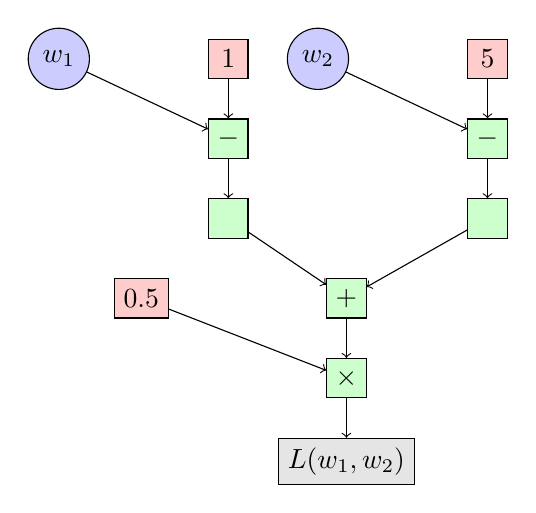
\begin{tikzpicture}[node distance=0.5cm, auto,
            input/.style={draw, circle, fill=blue!20, minimum size=0.5cm},
            const/.style={draw, rectangle, fill=red!20, minimum size=0.5cm},
            op/.style={draw, shape=rectangle, fill=green!20, inner sep=2pt, minimum width=0.5cm, minimum height=0.5cm},
            output/.style={draw, rectangle, fill=gray!20, minimum size=0.5cm}]
        
            % Layer 1: Inputs & constants for subtraction
            \node[input] (w1) {$w_1$};
            \node[input, right=2.5cm of w1] (w2) {$w_2$};
            \node[const, right=of w1, xshift=1.0cm] (c1) {1};
            \node[const, right=of w2, xshift=1.0cm] (c2) {5};
        
            % Layer 2: Subtraction operations
            \node[op, below=of c1] (sub1) {$-$};
            \node[op, below=of c2] (sub2) {$-$};
        
            % Layer 3: Squaring operations
            \node[op, below=of sub1] (sq1) {$\square$};
            \node[op, below=of sub2] (sq2) {$\square$};
        
            % Layer 4: Addition of squares
            \node[op, below=of sq1, xshift=1.5cm] (add) {$+$};
        
            % Layer 5: Constant for multiplication
            \node[const, left=of add, xshift=-1.5cm] (half) {0.5};
        
            % Layer 6: Multiplication to produce loss
            \node[op, below=of add] (mul) {$\times$};
        
            % Layer 7: Loss output
            \node[output, below=of mul] (loss) {$L(w_1, w_2)$};
        
            % Draw arrows from inputs to subtraction nodes
            \draw[->] (w1) -- (sub1);
            \draw[->] (c1) -- (sub1);
            \draw[->] (w2) -- (sub2);
            \draw[->] (c2) -- (sub2);
        
            % From subtraction to squaring
            \draw[->] (sub1) -- (sq1);
            \draw[->] (sub2) -- (sq2);
        
            % From squaring to addition
            \draw[->] (sq1) -- (add);
            \draw[->] (sq2) -- (add);
        
            % From multiplication constant and addition to multiplication node
            \draw[->] (half) -- (mul);
            \draw[->] (add) -- (mul);
        
            % Finally, multiplication to loss
            \draw[->] (mul) -- (loss);
        \end{tikzpicture}
    \end{center}
}

\frame{
    \frametitle{Computational Graphs: automatic differentiation}
    \begin{itemize}
        \item In the above example the loss function $L$ is a function of the parameters $w_1$ and $w_2$. In a neural network, the loss is a function of all the weights and biases in the network.
        \item We can then look at Neural networks as large computational graphs: input flows forward through layers to compute output, and we can trace how each weight influences the final loss.
        \item Deep learning frameworks (e.g. PyTorch, TensorFlow) build these graphs during the forward pass, recording operations and their inputs/outputs.
        \item This sets the stage for \textbf{automatic differentiation}.
        \item Automatic differentiation is a technique to compute the gradient of a function with respect to its inputs automatically using the \textbf{chain rule}.
    \end{itemize}
}


\frame{
    \frametitle{Chain Rule - The Engine of Backpropagation}
    \begin{itemize}
        \item \textbf{Chain Rule (Calculus):} If $y = f(u)$ and $u = g(x)$, then $\frac{dy}{dx} = \frac{dy}{du} \cdot \frac{du}{dx}$. For a composition of many functions, gradients multiply along the chain.
        \item In a computational graph, the chain rule allows us to propagate gradients backward: the gradient of a node's output w.r.t. some input equals the product of gradients along the path from input to output.
        \item \textbf{Local Gradients:} Each operation knows how its output changes w.r.t. its inputs. Backpropagation uses these local derivatives and the chain rule to get global gradients.
        \item \textbf{Key idea: Backpropagation} boils down to applying the chain rule repeatedly on a graph of computations.
    \end{itemize}
}

\frame{
    \frametitle{What is Backpropagation?}
    \begin{itemize}
        \item Backpropagation = “backward propagation of errors” - the core algorithm that computes the gradient of the loss with respect to all parameters in the model.
        \item It is essentially an efficient application of the chain rule on the computational graph of the model's forward pass. It allocates portions of the output error to each weight by traversing the graph in reverse.
        \item \textbf{Forward pass:} compute outputs and loss using current weights.
        \item \textbf{Backward pass:} starting from the loss, propagate the error gradient backward through each operation (layer) to find $\frac{\partial L}{\partial w}$ for every weight $w$.
        \item The result is the gradient vector given by $\nabla_\theta L$ (partial derivatives of loss w.r.t. each parameter collected in a vector $\theta$). We use this to update weights (e.g. using gradient descent).
    \end{itemize}
}

\frame{
    \frametitle{Backpropagation -- Step by Step}
    Consider the network
    \[
    f_\theta(x) = \sigma\Biggl(\sum_{k} \beta_k\, h_k(x) + b^{(2)}\Biggr)
    \quad\text{with}\quad
    h_k(x) = \sigma\Biggl(\sum_j w_{kj}\, x_j + b^{(1)}_k\Biggr).
    \]
    For a single data point \((x,y)\), define the loss as $L = \frac{1}{2}\bigl(y - f_\theta(x)\bigr)^2.$ $\sigma$ is the sigmoid function.
    \pause
    \begin{enumerate}
        \item \textbf{Forward Pass:}  
          Compute the prediction \(f_\theta(x)\) and store intermediate values (e.g. \(h_k(x)\) and \(z_k = \sum_j w_{kj}x_j + b^{(1)}_k\)).
          
        \item \textbf{Output Gradient:}  
          Initialize with \(\frac{\partial L}{\partial L} = 1\) and compute the gradient w.r.t. the output:
          \[
          \frac{\partial L}{\partial f_\theta(x)} = -(y - f_\theta(x)).
          \]
          
        \item \textbf{Backprop through Output Layer:}  
          For each output weight \(\beta_k\), compute
          \[
          \frac{\partial L}{\partial \beta_k} = \frac{\partial L}{\partial f_\theta(x)} \cdot h_k(x).
          \]
    \end{enumerate}
}


\frame{
    \frametitle{Backpropagation -- Step by Step (Cont.)}
    \begin{enumerate}
        \setcounter{enumi}{3}
        \item \textbf{Backprop through Hidden Layer:}  
          For each hidden weight \(w_{kj}\) (connecting input \(j\) to hidden unit \(k\)), recall that
          \[
          z_k = \sum_j w_{kj} x_j + b^{(1)}_k \quad\text{and}\quad h_k(x) = \sigma(z_k).
          \]
          Then, the gradient is given by
          \[
          \frac{\partial L}{\partial w_{kj}} = \frac{\partial L}{\partial f_\theta(x)} \cdot \beta_k \cdot \sigma'(z_k) \cdot x_j.
          \]
          
        \item \textbf{Extend to Deeper Layers:}  
          For networks with more layers, apply the chain rule recursively, propagating the error backwards.
          
        \item \textbf{Gradient Updates:}  
          Once the full gradient \(\nabla_\theta L\) is computed, update each parameter using gradient descent:
          \[
          \theta \leftarrow \theta - \alpha\, \nabla_\theta L.
          \]
    \end{enumerate}
}

\frame{
    \frametitle{Training with Backprop + Gradient Descent}
    Combine backprop with an iterative training loop: for each epoch (and for each batch of data):
    \begin{itemize}
        \item Forward pass: compute predictions and loss
        \item Backward pass: compute gradients via backpropagation
        \item Update weights: $w \gets w - \alpha \nabla_w L$ for all weights (using the chosen gradient descent variant)
        \item Batch GD: use all training data to compute an average gradient, then update once per epoch.
        \item Stochastic GD: update for each training example (one forward/backward per example).
        \item Mini-batch GD: update for each small batch (common in practice, e.g. 32 samples gives a good balance).
    \end{itemize}
    Iterate for many epochs - the loss typically decreases and the model improves. Backpropagation ensures each weight is nudged in the direction that most reduces the error.
    Outcome: The network's weights gradually converge to values that produce low loss (i.e., the network learns from the data).
}

\frame{
    \frametitle{Coding Demo: Building an Automatic Differentiation Engine}
    \begin{itemize}
        \item We will now build a simple automatic differentiation engine from scratch (in code) to illustrate backpropagation in action.
        \item This engine will construct a computational graph during the forward pass and then automatically compute gradients via backprop (chain rule) in the backward pass.
        \item We'll use it to optimize a small example by gradient descent - seeing how the code mirrors the math.
        %This hands-on approach follows Karpathy’s micrograd project, showing that with ~100 lines of code we can implement core backprop functionality!
    \end{itemize}
}




\end{document}